% !TeX program = pdflatex
% Standalone source. Compile with pdfLaTeX; no external figures are required.
\documentclass[11pt,a4paper]{article}
\usepackage[margin=20mm]{geometry}
\usepackage[T1]{fontenc}
\usepackage{lmodern}
\usepackage{amsmath,amssymb,booktabs,array,xcolor,tikz,fancyhdr,hyperref,listings,pgfplots}
\usetikzlibrary{calc,arrows.meta}
\hypersetup{colorlinks=true,linkcolor=blue!50!black,urlcolor=blue!50!black}
\definecolor{accent}{HTML}{124E66}
\definecolor{pcol}{HTML}{A24021}
\definecolor{ncol}{HTML}{175A86}
\pagestyle{fancy}\fancyhf{}\fancyhead[L]{\small EE3032 / Fall 2017 / HW4}
\fancyhead[R]{\small CMOS logic}\fancyfoot[C]{\thepage}
\setlength{\headheight}{15pt}\setlength{\parindent}{0pt}\setlength{\parskip}{6pt}
\renewcommand{\arraystretch}{1.2}
\newcommand{\answer}[1]{\par\noindent\colorbox{accent!9}{\parbox{0.96\linewidth}{#1}}\par}
\newcommand{\AND}{\,}
\newcommand{\VDD}{V_{\mathrm{DD}}}
\newcommand{\VSS}{V_{\mathrm{SS}}}
% A conventional switch-level MOS symbol: continuous channel, insulated gate,
% and a gate bubble for pMOS. Bulk terminals are omitted, as explained below.
% Arguments: device id, x, y, gate literal, p or n. t/b are upper/lower terminals.
\newcommand{\MOS}[5]{
  \coordinate (#1) at (#2,#3);
  \coordinate (#1t) at ($(#1)+(0,.55)$);
  \coordinate (#1b) at ($(#1)+(0,-.55)$);
  \draw (#1t)--($(#1)+(0,.30)$)--($(#1)+(-.18,.30)$);
  \draw ($(#1)+(-.18,.34)$)--($(#1)+(-.18,-.34)$);
  \draw ($(#1)+(-.18,-.30)$)--($(#1)+(0,-.30)$)--(#1b);
  \draw ($(#1)+(-.35,.33)$)--($(#1)+(-.35,-.33)$);
  \def\type{#5}\def\ptype{p}
  \ifx\type\ptype
    \draw ($(#1)+(-.78,0)$)--($(#1)+(-.53,0)$);
    \draw ($(#1)+(-.465,0)$) circle (.065);
    \draw ($(#1)+(-.40,0)$)--($(#1)+(-.35,0)$);
  \else
    \draw ($(#1)+(-.78,0)$)--($(#1)+(-.35,0)$);
  \fi
  \node[anchor=east] at ($(#1)+(-.82,0)$) {$#4$};
  \node[anchor=west,font=\scriptsize] at ($(#1)+(.10,0)$) {#1};
}
% A transmission-gate instance; its two MOS devices are expanded on page 3.
\newcommand{\TG}[4]{
  \node[draw,rounded corners=1pt,minimum width=11mm,minimum height=6mm,
        fill=accent!5,font=\small] (#1) at (#2,#3) {$\mathrm{TG}_{#4}$};
}

\pgfplotsset{compat=1.18}
\lstset{basicstyle=\ttfamily\scriptsize,breaklines=true,frame=single,columns=fullflexible}
\begin{document}
\begin{center}{\LARGE\bfseries 2017 HW4}\\[4pt]{\large Mirror and Domino CMOS Full Adders}\\[4pt]{\small EE3032 / Introduction to VLSI Design}\end{center}
The original full-adder prompt and supplied report/netlists were read first. Both requested pre-layout circuits are provided as runnable \texttt{.sp} designs and independently verified. The actual 2017 prompt asks no layout; this deliverable is entirely pre-layout.
\section*{1. Functions and verification conditions}
\[
 C_{out}=AB+AC+BC,\qquad S=A\oplus B\oplus C
 =(A+B+C)\bar C_{out}+ABC.
\]
\begin{center}\begin{tabular}{ccc|cc}\toprule
A&B&C&S&$C_{out}$\\\midrule
0&0&0&0&0\\0&0&1&1&0\\0&1&0&1&0\\0&1&1&0&1\\
1&0&0&1&0\\1&0&1&0&1\\1&1&0&0&1\\1&1&1&1&1\\\bottomrule
\end{tabular}\end{center}
Both designs use local CIC018 TT BSIM3 at 1.8 V,25$^\circ$C,100 ps input/clock ramps,1 fF on each output, and \texttt{DELMAX=2p}. PMOS bodies are VDD; NMOS bodies are VSS. All channel lengths are 0.18$\,\mu$m except the weak domino keepers (0.36$\,\mu$m).
\textbf{Meaning of $t_r=t_f$.} Rise/fall times mean output 10--90\%/90--10\% intervals. With different pull-network paths, one width cannot make every transition exactly identical. We therefore calibrate the maximum rise and maximum fall time for each output under the specified test set, and require less than 1\% mismatch. This is a stated finite-tolerance implementation of the prompt's balance target, not an unsupported equality at all inputs/process corners.
\begin{center}\begin{tabular}{llrrrr}\toprule
Design&Output&$t_r$ (ps)&$t_f$ (ps)&Mismatch (\%)&Worst delay (ps)\\\midrule
Mirror&S&55.403&54.956&0.806&256.205\\
Mirror&Cout&47.484&47.467&0.037&141.254\\
Domino&S&51.086&51.597&0.990&123.195\\
Domino&Cout&47.557&47.792&0.491&90.284\\
\bottomrule\end{tabular}\end{center}
For the mirror circuit, delay is from a primary-input 50\% crossing to the last output 50\% crossing in the transition window. For domino, evaluation delay is from CLK 50\% to output 50\%; precharge fall times are measured separately. These trigger definitions differ, so the two delay columns should not be treated as a direct unclocked speed comparison.
\newpage
\section*{2(a). 28-transistor mirror full adder}
The complementary carry node is $cb=\overline{C_{out}}$. Its PDN implements
$AB+C(A+B)$: one A--B series branch in parallel with C in series with A/B parallel devices. The dual PUN uses five pMOS. The sum complementary node is
\[
 sb=\overline{cb(A+B+C)+ABC}=\bar S.
\]
Its PDN has $cb$ in series with parallel A/B/C devices, in parallel with a three-device A--B--C stack (seven nMOS). The dual PUN has the corresponding seven pMOS. Two output inverters restore S and carry. Thus the graph has
\[
 5n+5p\ (carry)+7n+7p\ (sum)+2n+2p\ (outputs)=28\ MOSFETs.
\]
This is the original mirror graph, not a substitute XOR-chain full adder. Internal sizing compensates approximately for stack depth: two-device nMOS paths use 1.2$\,\mu$m widths and three-device paths use 1.8$\,\mu$m; corresponding pMOS use 3.6 and 5.4$\,\mu$m. Output nMOS widths are 0.6$\,\mu$m. Calibrated output pMOS widths are
\[
 W_{p,S}=2.727010\,\mu\mathrm m,\qquad
 W_{p,C}=2.017930\,\mu\mathrm m.
\]
Every directed transition between distinct three-bit words is tested: $8\times 7=56$. Data have 4.9 ns to settle in the old state, change over 100 ps, and then settle for 3.5 ns before sampling. Both output voltages pass in all 112 samples.64 intended output edges have their delay and slew recorded. Last-crossing extraction handles multiple-input hazards without reporting an early glitch as final propagation.
\textbf{Reference comparison.} The supplied report uses the same mirror structure and starts from an inverter width ratio 3.5 to balance that inverter at 1 V. It does not demonstrate balance across every full-adder transition. We retain the correct graph, use systematic stack sizing, and calibrate the actual output rise/fall maxima across all 56 transitions at the declared nominal 1.8 V condition.
\section*{2(b). Independent dual-rail domino full adder}
A single-rail domino gate is monotonic during evaluation, whereas S is non-unate in A/B/C. Generate stable complements $\bar A,\bar B,\bar C$ during precharge, then evaluate positive minterms in the six input rails:
\[
 S=\bar A\bar B C+\bar A B\bar C+A\bar B\bar C+ABC,
 \qquad C_{out}=AB+AC+BC.
\]
The dynamic carry node uses three parallel two-nMOS series paths. The dynamic sum node uses four parallel three-nMOS paths. Each node has its own clocked evaluation footer, clocked pMOS precharger, output inverter, and weak feedback keeper. Explicit 2 fF storage capacitance is added to each dynamic node to limit charge sharing. The three input-complement inverters bring the total to 34 MOSFETs.
\newpage
\textbf{Complete sum network.} The schematic below expands all four minterm stacks and the precharge, evaluation, keeper, and output devices. Inputs and their complements are stable throughout evaluation; all matching gate labels denote connected nets.
\begin{center}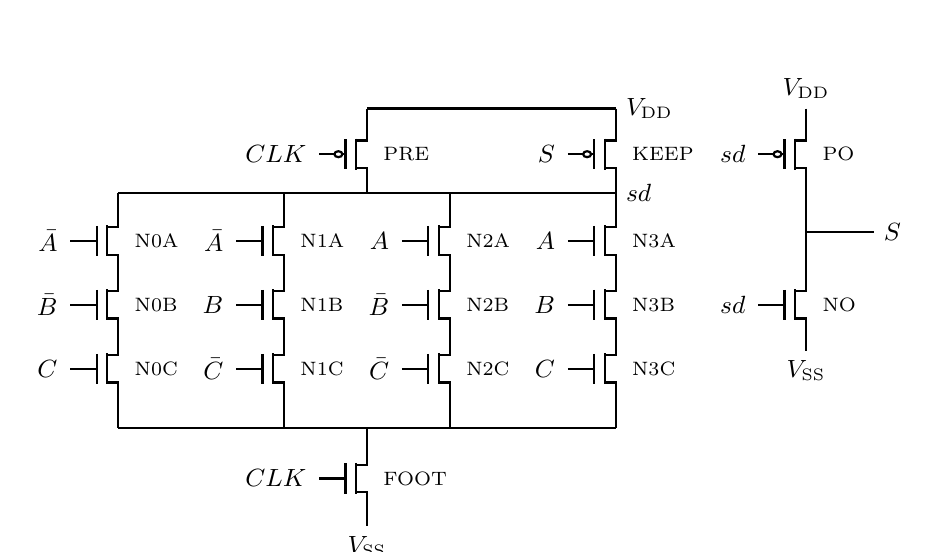
\begin{tikzpicture}[x=.78cm,y=.58cm,line width=.8pt,font=\small]
\MOS{PRE}{4.05}{6.5}{CLK}{p}\MOS{KEEP}{8.1}{6.5}{S}{p}
\draw (4.05,7.5)--(8.1,7.5) node[right] {$\VDD$};\draw (4.05,7.5)--(PREt) (8.1,7.5)--(KEEPt);
\draw (PREb)--(4.05,5.65) (KEEPb)--(8.1,5.65);\draw (0,5.65)--(8.1,5.65) node[right] {$sd$};
\MOS{N0A}{0}{4.6}{\bar A}{n}\MOS{N0B}{0}{3.2}{\bar B}{n}\MOS{N0C}{0}{1.8}{C}{n}
\MOS{N1A}{2.7}{4.6}{\bar A}{n}\MOS{N1B}{2.7}{3.2}{B}{n}\MOS{N1C}{2.7}{1.8}{\bar C}{n}
\MOS{N2A}{5.4}{4.6}{A}{n}\MOS{N2B}{5.4}{3.2}{\bar B}{n}\MOS{N2C}{5.4}{1.8}{\bar C}{n}
\MOS{N3A}{8.1}{4.6}{A}{n}\MOS{N3B}{8.1}{3.2}{B}{n}\MOS{N3C}{8.1}{1.8}{C}{n}
\foreach \i/\x in {0/0,1/2.7,2/5.4,3/8.1}{\draw (\x,5.65)--(N\i At) (N\i Ab)--(N\i Bt) (N\i Bb)--(N\i Ct) (N\i Cb)--(\x,.5);}
\draw (0,.5)--(8.1,.5);\MOS{FOOT}{4.05}{-.6}{CLK}{n}
\draw (4.05,.5)--(FOOTt) (FOOTb)--(4.05,-1.65) node[below] {$\VSS$};
\MOS{PO}{11.2}{6.5}{sd}{p}\MOS{NO}{11.2}{3.2}{sd}{n}
\draw (11.2,7.5) node[above] {$\VDD$}--(POt) (POb)--(NOt);\draw (11.2,4.8)--(12.3,4.8) node[right] {$S$};\draw (NOb)--(11.2,2.2) node[below] {$\VSS$};
\end{tikzpicture}\end{center}
Carry uses three parallel series pairs: A--B, A--C, and B--C. Its precharger, footer, keeper, and output inverter have the same roles as in the sum gate. The complete source listings below specify every transistor and width.
Sum-stack nMOS widths are 2.4$\,\mu$m, carry-stack nMOS widths 1.8$\,\mu$m, footers 3.6$\,\mu$m, keeper pMOS widths 0.3$\,\mu$m with L=0.36$\,\mu$m, and output inverter widths $(W_p,W_n)=(2.1,0.6)\,\mu$m. Precharge sizing balances reset fall time against evaluate rise time:
\[
 W_{pre,S}=3.108270\,\mu\mathrm m,\qquad
 W_{pre,C}=2.495240\,\mu\mathrm m.
\]
\textbf{Clock protocol.} CLK=0 precharges both dynamic nodes high and resets both outputs to 0. Data changes at 1--1.1 ns within each 10 ns cycle; CLK rises at 5--5.1 ns, after the true/complement rails settle. CLK is high for 4 ns, then falls over 100 ps. During high CLK, inputs hold their values. Thus no input rail falls during the evaluate phase.
Every one of the eight input words is independently evaluated after precharge. All 16 evaluate output samples and all 16 precharge/reset samples pass the rail bounds (low $\le 0.2$ V, high $\ge 1.6$ V). There are eight output evaluation rises and eight reset falls. Zero outputs are verified as stable lows; they do not have an evaluation propagation edge.
\textbf{Reference correction.} The supplied domino sum uses the raw falling dynamic carry-complement node as an nMOS gate. That select starts high in precharge and falls during evaluation; it can discharge the sum node before carry resolves, and a dynamic node cannot recharge during evaluation. The supplied report observes nonzero sum for two two-one input words. Our independent minterms avoid that falling-select dependency. Weak keepers and declared storage capacitors address charge sharing, and every state is checked using settled precharge data.
\newpage
\section*{3. Worst-case transition evidence}
\begin{center}\begin{tabular}{llllr}\toprule
Design&Output&Transition&Edge&Worst delay (ps)\\\midrule
Mirror&S&110$\to$100&rise&256.205\\
Mirror&Cout&000$\to$110&rise&141.254\\
Domino&S&000$\to$010&rise&123.195\\
Domino&Cout&000$\to$110&rise&90.284\\
\bottomrule\end{tabular}\end{center}
For domino, ``000'' in the old-state column means reset outputs 0; each listed new word is evaluated independently after precharge. It is not a direct asynchronous data transition. The calibrated maxima and complete matrices are in \texttt{results/}; raw HSPICE outputs remain in the chosen work directory.
\textbf{Reproduce.} Run \texttt{python reproduce.py --model D:/cic018.l --work PATH --no-calibrate} to verify the saved calibrated dimensions. Omit \texttt{--no-calibrate} to allow further automatic rise/fall balancing. \texttt{--hspice PATH} selects the installed simulator. The program stops on license/simulation errors, failed rail checks, missing crossings, or failure of the 1\% balance target.
\texttt{mirror\_sizes.json} and \texttt{domino\_sizes.json} record the dimensions. The same calibrated defaults are persisted into the delivered subcircuits. The two testbenches are standalone runs with the required process file kept local. No layout, extraction, or proprietary process-model text is distributed.
\section*{4. Complete mirror netlist}
\begin{lstlisting}
* 28T mirror full adder. Explicit VDD/VSS and bulk terminals.
.param WOSC=2.017930000u WOSS=2.727010000u
.subckt mirror_fa a b c s co vdd vss
* Complementary carry node cb = NOT(AB + C(A+B)).
MPA1 cp1 a vdd vdd P_18 w=3.6u l=.18u
MPB1 cp1 b vdd vdd P_18 w=3.6u l=.18u
MPC1 cb c cp1 vdd P_18 w=3.6u l=.18u
MPA2 cp2 a vdd vdd P_18 w=3.6u l=.18u
MPB2 cb b cp2 vdd P_18 w=3.6u l=.18u
MNA1 cn1 a vss vss N_18 w=1.2u l=.18u
MNB1 cn1 b vss vss N_18 w=1.2u l=.18u
MNC1 cb c cn1 vss N_18 w=1.2u l=.18u
MNA2 cn2 a vss vss N_18 w=1.2u l=.18u
MNB2 cb b cn2 vss N_18 w=1.2u l=.18u
* Complementary sum: discharge predicate cb(A+B+C)+ABC.
MPA3 sp1 a vdd vdd P_18 w=3.6u l=.18u
MPB3 sp1 b vdd vdd P_18 w=3.6u l=.18u
MPC2 sp1 c vdd vdd P_18 w=3.6u l=.18u
MPU sb cb sp1 vdd P_18 w=3.6u l=.18u
MPA4 sp2 a vdd vdd P_18 w=5.4u l=.18u
MPB4 sp3 b sp2 vdd P_18 w=5.4u l=.18u
MPC3 sb c sp3 vdd P_18 w=5.4u l=.18u
MNA3 sn1 a vss vss N_18 w=1.2u l=.18u
MNB3 sn1 b vss vss N_18 w=1.2u l=.18u
MNC2 sn1 c vss vss N_18 w=1.2u l=.18u
MND sb cb sn1 vss N_18 w=1.2u l=.18u
MNA4 sn2 a vss vss N_18 w=1.8u l=.18u
MNB4 sn3 b sn2 vss N_18 w=1.8u l=.18u
MNC3 sb c sn3 vss N_18 w=1.8u l=.18u
* Separately calibrated output inverters.
MPOC co cb vdd vdd P_18 w=WOSC l=.18u
MNOC co cb vss vss N_18 w=.6u l=.18u
MPOS s sb vdd vdd P_18 w=WOSS l=.18u
MNOS s sb vss vss N_18 w=.6u l=.18u
.ends mirror_fa
\end{lstlisting}
\newpage
\section*{5. Complete domino netlist}
\begin{lstlisting}
* Robust dual-rail domino full adder. Data stable before CLK rises.
* No falling dynamic carry node drives the sum NMOS gates.
.param WPSC=2.495240000u WPSS=3.108270000u
.subckt domino_fa a b c clk s co vdd vss
* Static complements settle during precharge.
MPA ab a vdd vdd P_18 w=1.8u l=.18u
MNA ab a vss vss N_18 w=.6u l=.18u
MPB bb b vdd vdd P_18 w=1.8u l=.18u
MNB bb b vss vss N_18 w=.6u l=.18u
MPC cb c vdd vdd P_18 w=1.8u l=.18u
MNC cb c vss vss N_18 w=.6u l=.18u
* Independent dynamic carry; co=AB+AC+BC.
MPREC cd clk vdd vdd P_18 w=WPSC l=.18u
MNCA cd a cn1 vss N_18 w=1.8u l=.18u
MNCB cn1 b cf vss N_18 w=1.8u l=.18u
MNCC cd a cn2 vss N_18 w=1.8u l=.18u
MNCD cn2 c cf vss N_18 w=1.8u l=.18u
MNCE cd b cn3 vss N_18 w=1.8u l=.18u
MNCF cn3 c cf vss N_18 w=1.8u l=.18u
MNFC cf clk vss vss N_18 w=3.6u l=.18u
MPKC cd co vdd vdd P_18 w=.3u l=.36u
MPOC co cd vdd vdd P_18 w=2.1u l=.18u
MNOC co cd vss vss N_18 w=.6u l=.18u
* Independent dynamic sum: ab*bb*c + ab*b*cb + a*bb*cb + a*b*c.
MPRES sd clk vdd vdd P_18 w=WPSS l=.18u
MNS0A sd ab sn0a vss N_18 w=2.4u l=.18u
MNS0B sn0a bb sn0b vss N_18 w=2.4u l=.18u
MNS0C sn0b c sf vss N_18 w=2.4u l=.18u
MNS1A sd ab sn1a vss N_18 w=2.4u l=.18u
MNS1B sn1a b sn1b vss N_18 w=2.4u l=.18u
MNS1C sn1b cb sf vss N_18 w=2.4u l=.18u
MNS2A sd a sn2a vss N_18 w=2.4u l=.18u
MNS2B sn2a bb sn2b vss N_18 w=2.4u l=.18u
MNS2C sn2b cb sf vss N_18 w=2.4u l=.18u
MNS3A sd a sn3a vss N_18 w=2.4u l=.18u
MNS3B sn3a b sn3b vss N_18 w=2.4u l=.18u
MNS3C sn3b c sf vss N_18 w=2.4u l=.18u
MNFS sf clk vss vss N_18 w=3.6u l=.18u
MPKS sd s vdd vdd P_18 w=.3u l=.36u
MPOS s sd vdd vdd P_18 w=2.1u l=.18u
MNOS s sd vss vss N_18 w=.6u l=.18u
* Explicit storage capacitance to limit charge sharing.
CSD sd vss 2f
CCD cd vss 2f
.ends domino_fa
\end{lstlisting}
\end{document}
